\documentclass[a4paper]{article}
\usepackage[utf8]{vntex}
%\usepackage[english,vietnam]{babel}
%\usepackage[utf8]{inputenc}
\usepackage{mathptmx}[ptm]
%\usepackage[utf8]{inputenc}
%\usepackage[francais]{babel}
\usepackage{a4wide,amssymb,epsfig,latexsym,array,hhline,fancyhdr}
\usepackage[normalem]{ulem}
%\usepackage{soul}

\usepackage[makeroom]{cancel}
\usepackage{amsmath}
\usepackage{amsthm}
\usepackage{multicol,longtable,amscd}
\usepackage{diagbox}%Make diagonal lines in tables
\usepackage{booktabs}
\usepackage{alltt}
\usepackage[framemethod=tikz]{mdframed}% For highlighting paragraph backgrounds
\usepackage{caption,subcaption}

\usepackage{lastpage}
\usepackage[lined,boxed,commentsnumbered]{algorithm2e}
\usepackage{enumerate}
\usepackage{color}
\usepackage{graphicx}							% Standard graphics package
\usepackage{array}
\usepackage{tabularx, caption}
\usepackage{multirow}
\usepackage{multicol}
\usepackage{rotating}
\usepackage{graphics}
\usepackage{geometry}
\usepackage{setspace}
\usepackage{epsfig}
\usepackage{tikz}
\usepackage{algorithm2e}
\usepackage{algorithm}
\usepackage{algorithmic}

\usetikzlibrary{arrows,snakes,backgrounds,calc,intersections}
\usepackage[unicode]{hyperref}
\hypersetup{urlcolor=blue,linkcolor=black,citecolor=black,colorlinks=true} 
\usepackage{listings}

%\usepackage{pstcol} 								% PSTricks with the standard color package

\usepackage[normalem]{ulem}

\newtheorem{definition}{\bf Định nghĩa}
\newtheorem{theorem}{{\bf Định lý}}
\newtheorem{property}{{\bf Tính chất}}
\newtheorem{proposition}{{\bf Mệnh đề}}
\newtheorem{corollary}[proposition]{{\bf Hệ quả}}
\newtheorem{lemma}[proposition]{{\bf Bổ đề}}
\theoremstyle{definition}
\newtheorem{exer}{Bài toán}
\addtocontents{toc}{\protect\thispagestyle{empty}}
% Remove page number in contents page. 
\addtocontents{lof}{\protect\thispagestyle{empty}}
% Remove page number in list of figure page. 
\addtocontents{lot}{\protect\thispagestyle{empty}}
% Remove page number in list of table page. 
\def\thesislayout{	% A4: 210 × 297
	\geometry{
		a4paper,
		total={160mm,240mm},  % fix over page
		left=30mm,
		top=22mm,
            right=20mm,
            bottom=20mm,
	}
}
\def\thesisheadlayout{	% A4: 210 × 297
	\geometry{
		a4paper,
		total={160mm,240mm},  % fix over page
		left=30mm,
		top=10mm,
	}
}
\thesislayout
\lstset{
language=R,
basicstyle=\footnotesize\sffamily,
commentstyle=\ttfamily\color{black},
numbers=left,
numberstyle=\ttfamily\color{black}\footnotesize,
stepnumber=1,
numbersep=5pt,
backgroundcolor=\color{white},
showspaces=false,
showstringspaces=false,
showtabs=false,
frame=single,
tabsize=2,
captionpos=b,
breaklines=true,
breakatwhitespace=false,
title=\lstname,
escapeinside={},
keywordstyle={},
morekeywords={}
}
%\usepackage{fancyhdr}
\setlength{\headheight}{40pt}
\pagestyle{fancy}
\fancyhead{} % clear all header fields
\renewcommand{\footruleskip}{1mm}

\fancyhead[L]{
 \begin{tabular}{rl}
    \begin{picture}(25,15)(0,0)
    \put(0,-8){\includegraphics[width=10mm, height=10mm]{Images/1-hcmut.png}}
    %\put(0,-8){\epsfig{width=10mm,figure=hcmut.eps}}
   \end{picture}&
	%\includegraphics[width=8mm, height=8mm]{hcmut.png} & %
	\begin{tabular}{l}
		\textbf{  Trường Đại Học Bách Khoa - Đại học Quốc gia TP.HCM }\\
		%\textbf{  Khoa Điện - Điện tử}
	\end{tabular} 	
 \end{tabular}
}
\fancyhead[R]{
	\begin{tabular}{l}
		\tiny \bf \\
		\tiny \bf 
	\end{tabular}  }
\fancyfoot{} % clear all footer fields
\fancyfoot[L]{\scriptsize  Báo cáo Bài tập lớn/Môn Phương pháp tính - HK2 2024 - 2025}
\fancyfoot[R]{\scriptsize  Trang {\thepage}/\pageref{LastPage}}

\renewcommand{\headrulewidth}{0.3pt}
\renewcommand{\footrulewidth}{0.3pt}

%%%
\setcounter{secnumdepth}{4}
\setcounter{tocdepth}{3}
\makeatletter
\newcounter {subsubsubsection}[subsubsection]
\renewcommand\thesubsubsubsection{\thesubsubsection .\@alph\c@subsubsubsection}
\newcommand\subsubsubsection{\@startsection{subsubsubsection}{4}{\z@}%
                                     {-3.25ex\@plus -1ex \@minus -.2ex}%
                                     {1.5ex \@plus .2ex}%
                                     {\normalfont\normalsize\bfseries}}
\newcommand*\l@subsubsubsection{\@dottedtocline{3}{10.0em}{4.1em}}
\newcommand*{\subsubsubsectionmark}[1]{}
\makeatother

\everymath{\color{black}}%make in-line maths symbols blue to read/check easily

\sloppy
\captionsetup[figure]{labelfont={small,bf},textfont={small,it},belowskip=-1pt,aboveskip=-9pt}
%space remove between caption, figure, and text
\captionsetup[table]{labelfont={small,bf},textfont={small,it},belowskip=-1pt,aboveskip=7pt}
\setlength{\floatsep}{5pt plus 2pt minus 2pt}
\setlength{\textfloatsep}{5pt plus 2pt minus 2pt}
\setlength{\intextsep}{10pt plus 2pt minus 2pt}

\thesislayout

\begin{document}

\begin{titlepage}
\begin{tikzpicture}[remember picture, overlay]
  \draw[line width = 4pt] ($(current page.north west) + (0.4in,-0.5in)$) rectangle ($(current page.south east) + (-0.4in,0.5in)$);
  \draw[line width=1.5pt]
    ($ (current page.north west) + (0.45in,-0.55in) $)
    rectangle
    ($ (current page.south east) + (-0.45in,0.55in) $);
\end{tikzpicture}

\begin{center}
\LARGE \textbf{ĐẠI HỌC QUỐC GIA THÀNH PHỐ HỒ CHÍ MINH} \\
\vspace{0.2cm}
\LARGE \textbf{TRƯỜNG ĐẠI HỌC BÁCH KHOA} \\
\vspace{0.2cm}
\LARGE \textbf{KHOA ĐIỆN - ĐIỆN TỬ}
\end{center}

\vspace{0.3cm}

\begin{figure}[h!]
\begin{center}
\includegraphics[width=4cm]{Images/1-hcmut.png}
\end{center}
\end{figure}

\begin{center}
\begin{tabular}{c}
\multicolumn{1}{c}{\textbf{{\LARGE BÁO CÁO}}}\\
\\{\textbf{{\LARGE BÀI TẬP LỚN}}}
\\{\textbf{{\LARGE MÔN HỌC PHƯƠNG PHÁP TÍNH}}}
\\ \textit{(MT1009)}
\\
\\
\textbf{\LARGE ĐỀ TÀI 14}\\
\textbf{\Large Finding shortest paths for autonomous robots in 2D and 2,5D }

\end{tabular}
\end{center}
\vspace{0.5cm}
\begin{table}[h]
\begin{tabular}{rll}
\hspace{2 cm} &  \textbf{\Large GVHD:} {\Large ................................}
\\
\\
\hspace{2 cm} &   \textbf{\Large Lớp:} {\Large AN01}
\\
\\
\hspace{2 cm}  &   \textbf{\Large Nhóm số:} {\Large 02}
\\
\\
\end{tabular}
\end{table}

\begin{center}
\vspace{0.5cm}

\textbf{\large Danh sách thành viên:}

\vspace{0.5cm}

% Increase row height by 2.5 times
\renewcommand{\arraystretch}{2}
\begin{tabular}{|c|m{8cm}|c|}
    \hline
    \textbf{STT} & \textbf{Họ và tên} & \textbf{MSSV} \\
    \hline
    1 & Lưu Gia Huy & 2411194\\
    \hline
    2 & Lê Đức Minh & 2414110\\
    \hline
    3 & & \\
    \hline
    4 & & \\
    \hline
\end{tabular}
\end{center}


\vspace{0.5cm}
\begin{center}
{\Large TP. HỒ CHÍ MINH, 2025 }
\end{center}
\end{titlepage}
%\thispagestyle{empty}
\newpage
%%%%%%%%%%%%%%%%%INTRO%%%%%%%%%%%%%%%%%%%
\input{Intro/1-LoiMoDau}
\input{Intro/2-LoiCamOn}
\input{Intro/3-TomTat}
\newpage
\tableofcontents
\newpage
\listoffigures
\newpage
\listoftables
\newpage
\setcounter{page}{1}

%%%%%%%%%%%%%%%%%CONTENTS%%%%%%%%%%%%%%%%%%%
\section{Giới thiệu}
\subsection{Giới thiệu đề tài}
Trong lập trình Robot tự động, việc tìm đường đi ngắn nhất giữa hai điểm giúp tiết kiệm tài nguyên, năng lượng, và thời gian. Điều này không chỉ nâng cao hiệu suất làm việc của Robot mà còn tối ưu hóa lợi nhuận trong nhiều ứng dụng thực tế. 

Trong bài viết này, nhóm chúng em sẽ nghiên cứu và triển khai thuật toán của D. T. Lee và F. P. Preparata nhằm tìm đường đi ngắn nhất trong một đa giác đơn (\textit{simple polygon}). Thuật toán này giúp cải thiện đáng kể thời gian xử lý so với các phương pháp truyền thống, có nhiều ứng dụng trong lĩnh vực robot tự động và điều hướng thông minh.

\subsection{Các hướng giải quyết liên quan}

Bài toán tìm đường đi ngắn nhất giữa hai điểm phân biệt ($s$: điểm bắt đầu, $t$: điểm kết thúc) trong mặt phẳng 2D là một trong những bài toán quan trọng của lý thuyết đồ thị và hình học tính toán. Có nhiều phương pháp tiếp cận bài toán này, trong đó phương pháp cổ điển sử dụng thuật toán Dijkstra trên đồ thị visbility graph, với độ phức tạp $O(n^2)$.

Tuy nhiên, thuật toán của Lee và Preparata cho phép tìm đường đi ngắn nhất trong một đa giác đơn với thời gian $O(n)$ nếu bỏ qua bước tiền xử lý tam giác hóa. Như vậy, tổng độ phức tạp của thuật toán phụ thuộc vào quá trình tam giác hóa đa giác. Hiện nay, đã có những nghiên cứu chỉ ra rằng có thể tam giác hóa một đa giác đơn trong thời gian $O(n)$ \cite{Triangulate_linear}. Do đó, thuật toán Lee và Preparata kết hợp với phương pháp tam giác hóa nhanh có thể là một giải pháp hiệu quả để giải quyết bài toán này.
\newpage
\section{Cơ sở lý thuyết}
\subsection{Các định nghĩa và bổ đề}% co khi xoa 2 cai subsection luon cung duoc}
Phần này giới thiệu một số định nghĩa sẽ được sử dụng trong bài:

\begin{definition}
    Một chuỗi đa giác\footnote{Từ nguyên: polygonal chain} $P = \overline{q_1 q_2 \cdots q_k}$ là chuỗi của các điểm $q_i (i=1, 2, \cdots, k)$ với mỗi cặp $q_i$ và $q_{i+1}$ là một đoạn thẳng và không có hai đoạn thẳng không liên tiếp nào cắt nhau.
\end{definition}

\begin{definition}
    Một đa giác đơn\footnote{Từ nguyên: simple polygon} $n$ đỉnh $P=\left(q_1, q_2, \cdots,q_n\right)$ là một chuỗi đa giác $\overline{q_1 q_2 \cdots q_{n+1}}$ với $q_{n+1} = q_1$. Đường chéo của $P$ là đoạn thẳng $\overline{q_i q_j}, j\ne i + 1$ và không cắt bất kỳ cạnh nào của $P$. Khi đó $P$ được coi như đã \textit{tam giác hóa} nếu phần bên trong nó được chia thành $n-2$ tam giác bởi $n-3$ đường chéo.
\end{definition}

Các đa giác đơn đã tam giác hóa có một tính chất thú vị như sau: Chúng ta có thể xem như đa giác đó là một đồ thị phẳng $G$ trong cùng mặt phẳng. Mỗi tam giác là một miền trong\footnote{Từ nguyên: interior face} của $G$. Từ đó xây dựng đồ thị đối ngẫu $G^D$ của $G$, mỗi mặt của $G$ là một điểm của $G^D$ và mỗi cạnh của $G^D$ được nối từ hai điểm mà mặt của chúng có cạnh chung trong $G$. Khi bỏ đi các điểm thuộc miền ngoài, $G^D$ trở thành một cây (tree) với các đỉnh có bậc tối đa là 3:

\begin{definition}
    Dual tree\footnote{Tạm dịch: cây đối ngẫu} của một đa giác đơn đã tam giác hóa $P$ là một đồ thị $T=(V,E)$ sao cho mỗi nút $V$ tương ứng với một tam giác của $P$ và mỗi cạnh của $E$ được nối bởi hai điểm khác nhau thuộc $V$ nếu tam giác tương ứng của chúng có cạnh chung là một đường chéo của $P$. Đường chéo của $P$ và cạnh tương ứng của $E$ trong $T$ được gọi là \textit{dual}.
\end{definition}


\begin{figure}[h] % h: here, t: top, b: bottom, p: page of floats
  \centering
 \begin{tikzpicture}[scale = 0.65]
%coordinate
    \coordinate (a) at (0,0); \coordinate (b) at (2, 2.5);
    \coordinate (c) at (0,7); \coordinate (d) at (0,13);
    \coordinate (e) at (2, 6); \coordinate (f) at (4.5, 6.25);
    \coordinate (g) at (8, 8.5); \coordinate (h) at (3, 9);
    \coordinate (i) at (5, 12); \coordinate (j) at (12, 10);
    \coordinate (k) at (13,0); \coordinate (l) at (9,0.25);
    \coordinate (m) at (8, 4); \coordinate (n) at (5,0);
    \coordinate (t1) at (0.5, 9); \coordinate (t2) at (1.5, 5);
    \coordinate (t3) at (3, 5.5); \coordinate (t4) at (5, 4.5);
    \coordinate (t5) at (5, 2); \coordinate (t6) at (3, 1);
    \coordinate (t7) at (5, 10); \coordinate (t8) at (8, 10.5);
    \coordinate (t9) at (9,8); \coordinate (t10) at (7, 7);
    \coordinate (t11) at (11, 7); \coordinate (t12) at (10,1);
    \coordinate (s) at (1,5.75); \coordinate (t) at (9.5, 1.5);
%polygon
    \draw[thick] (a) -- (b) -- (c) -- (d) -- (e) -- (f) -- (g) -- (h) -- (i) -- (j) -- (k) -- (l) --(m) -- (n) -- (a);
%diagonal
    \draw[thick, dashed] (c) -- (e); \draw[very thick, dashed] (e) -- (b) node[midway, fill=white] {$d_1$};
    \draw[very thick, dashed] (b) -- (f) node[midway, fill=white] {$d_2$}; \draw[thick, dashed] (b) -- (n);
    \draw[thick, dashed] (b) -- (m); \draw[very thick, dashed] (f) -- (m) node[midway, fill=white] {$d_3$};
    \draw[very thick, dashed] (g) -- (m) node[midway, fill=white] {$d_4$}; \draw[thick, dashed] (g) -- (i);
    \draw[thick, dashed] (g) -- (j); \draw[very thick, dashed] (m) -- (k) node[midway, fill=white] {$d_6$};
    \draw[very thick, dashed] (m) -- (j) node[midway, fill=white] {$d_5$};
%dual tree
    \draw[very thick] (t1) -- (t2) -- (t3) -- (t4) -- (t4) -- (t10) -- (t9) -- (t11) -- (t12);
    \draw[very thick] (t4) -- (t5) -- (t6);
    \draw[very thick] (t9) -- (t8) -- (t7);
%node
    \filldraw[white] (t1) circle (3pt); \draw[thick] (t1) circle (3pt);
    \filldraw[white] (t2) circle (3pt); \draw[thick] (t2) circle (3pt);
    \filldraw[white] (t3) circle (3pt); \draw[thick] (t3) circle (3pt);
    \filldraw[white] (t4) circle (3pt); \draw[thick] (t4) circle (3pt);
    \filldraw[white] (t5) circle (3pt); \draw[thick] (t5) circle (3pt);
    \filldraw[white] (t6) circle (3pt); \draw[thick] (t6) circle (3pt);
    \filldraw[white] (t7) circle (3pt); \draw[thick] (t7) circle (3pt);
    \filldraw[white] (t8) circle (3pt); \draw[thick] (t8) circle (3pt);
    \filldraw[white] (t9) circle (3pt); \draw[thick] (t9) circle (3pt);
    \filldraw[white] (t10) circle (3pt); \draw[thick] (t10) circle (3pt);
    \filldraw[white] (t11) circle (3pt); \draw[thick] (t11) circle (3pt);
    \filldraw[white] (t12) circle (3pt); \draw[thick] (t12) circle (3pt);
    \filldraw[black] (s) circle (3pt) node[above] {$s$};
    \filldraw[black] (t) circle (3pt) node[anchor = north east] {$t$};
%sleeve
    \draw[line width = 2.5pt] (e) -- (f) -- (g) -- (j) -- (k);
    \draw[line width = 2.5pt] (b) -- (m);
    \draw[line width = 2.5pt, dash dot] (e) -- (s) -- (b);
    \draw[line width = 2.5pt, dash dot] (m) -- (t) -- (k);
%arrows
    \draw[thick, latex-] (12.4,6) to [bend right] (14,7) node[above] {Sleeve $P'$};
    \draw[thick, latex-] (8.5, 11) to [bend left] (10,12) node[right] {Đa giác $P$};
    \draw[thick, latex-] (t12) ++(1,-0.5) to [bend right] (13.5,2) node[above] {$\Delta (t)$};
    \draw[thick, latex-] (s) ++(-0.25,0.25) to [bend right] (-0.5,7) node[left] {$\Delta (s)$};
    \draw[thick, latex-] (6.2,6) to [bend left] (4, 7.3) node[above] {Dual tree $G^D$ của $P$};
%buffer
    \filldraw[white] (-1,-1) circle (2pt);
\end{tikzpicture}
  \caption{Đa giác đã tam giác hóa và dual tree của nó.}
  \label{fig:1} % Optional label for referencing
\end{figure} 






Cần chú ý rằng có vô số cách để tam giác hóa một đa giác đơn và một trong những thuật toán sử dụng trong bài này sử dụng thuật toán $O\left(n \log n\right)$ \cite{Triangulate_nlogn}.

Phương pháp của Lee và Preparata dựa trên quan sát sau: Gọi $\Delta (s)$ và $\Delta (t)$ lần lượt là hai tam giác trong $P$ chứa $s, t$ tương ứng. Trong $T$, tồn tại duy nhất đường đi $\pi$ qua các đỉnh của $T$ là các đối ngẫu của $\Delta (s)$ và $\Delta (t)$. Các cạnh trong $\pi$ là đối ngẫu của các đường chéo trong $P$ nên chuỗi các cạnh này tương ứng là chuỗi các đường chéo $d_1, d_2, \cdots,d_p$ theo thứ tự từ $s$ tới $t$. Vì $d_i$ bất kỳ chia $P$ thành hai phần, một chứa $s$ và một chứa $t$ nên đường đi ngắn nhất từ $s$ tới $t$ trong $P$ sẽ phải đi ngang qua mỗi đường chéo $d_1, d_2, \cdots,d_p$ một lần duy nhất. Ta có bổ đề sau (Chứng minh \cite{Lee_paper_proof_lemma_1}):

\begin{lemma}
    Gọi $S$ là tập hợp các đầu mút của các \textit{rào chắn thẳng hàng}. Các đỉnh của đường đi ngắn nhất giữa $s$ và $t$ thuộc $S\cup \left\{s,t\right\}.$
\end{lemma}

Trong trường hợp này, $S$ là tập hợp các đỉnh của $P$. Bồ đề 1 nói ta chỉ cần dựng đường ngắn nhất từ $s$ tới hai đỉnh lần lượt của $d_1, d_2, ...,d_p$ và cuối cùng tới $t$. Hợp của các đường này gọi là cây đường đi ngắn nhất\footnote{Từ nguyên: shortest-path tree} với gốc là $s$. Bởi vì mỗi đường đi từ $s$ đều đi qua một đường chéo một lần duy nhất, ta sẽ đi xây dựng thuật toán tham lam\footnote{Từ nguyên: greedy algorithm}: xét các tam giác lần lượt trên $\pi$, với mỗi tam giác, ta mở rộng cây đường đi ngắn nhất thêm một cạnh và một đỉnh.


\subsection{Thuật toán đề xuất}
Phần này nói về thuật toán tìm được đi ngắn nhất giữa $s$ và $t$ bên trong $P$ thông qua thuật toán mở rộng cây đường đi ngắn nhất từng cạnh một. Bắt đầu với định nghĩa sau:
\begin{definition}
    Một đa giác đã tam giác hóa được gọi là \textit{sleeve}\footnote{Tạm dịch: tay áo} nếu cây đối ngẫu của nó là một chuỗi.
\end{definition}

Với định nghĩa này, ta xây dựng đa giác $P'$ đối ngẫu với $\pi$ sao cho $s, t$ là các đỉnh của đa giác $P'$. Trong phần tiếp theo,  ta sẽ giả sử rằng đa giác $P$ là một sleeve với $n$ đỉnh bao gồm $s$ và  $t$.  

Gọi $v^{(1)}_i$ và $v^{(2)}_i$ lần lượt là hai đầu mút của đường chéo $d_i, 1 \le i \le n -3$,  và gọi $D\left(s, v^{(j)}_i\right)$ là đường đi ngắn nhất từ $s$ tới $v^{(j)}_i, j = 1, 2$ bên trong đa giác $P$. Từ \ref{} $D\left(s, v^{(j)}_i\right)$ là chuỗi bao gồm các đỉnh của  $P$. Gọi $D_i = D\left(s, v^{(1)}_i\right) \cup D\left(s, v^{(2)}_i\right)$, trong $D_i$ tồn tại duy nhất một đỉnh $v$ là đỉnh chung của cả $D\left(s, v^{(1)}_i\right) $ và $ D\left(s, v^{(2)}_i\right)$, và $v$ cách $s$ xa nhất (theo các chuỗi); hay là hai chuỗi $D\left(s, v^{(1)}_i\right) $ và $ D\left(s, v^{(2)}_i\right)$ tách ra tại $v$. 

Giả sử ban đầu không có chuỗi $D$ nào rỗng; ta thấy rằng: $D\left(v, v^{(j)}_i\right) (j=1,2)$ là một chuỗi đa giác lồi vào trong\footnote{Từ nguyên: inward-convex}; nghĩa là phần lồi của nó hướng vào bên trong $P$.  

\begin{proof}
    Xét miền $R_i$  giới hạn bởi $D\left(v, v^{(1)}_i\right), D\left(v, v^{(2)}_i\right)$ và $d_i$  gọi là \textit{phễu}\footnote{Từ nguyên: funnel} nằm trong $P$. Gọi $d_s, d_{s+1}, \cdots, d_{i-1}$ là các đường chéo cắt $D\left(v, v^{(1)}_i\right), D\left(v, v^{(2)}_i\right)$. Dễ thấy tam giác $\left(v, v^{(1)}_s, v^{(2)}_s\right) = R_S$  nằm trong $P$, theo phương pháp quy nạp thì $R_{i-1} \subset P$. Nếu $D\left(v, v^{(1)}_i\right)$ không lồi vào trong, theo bất đẳng thức tam giác, tồn tại một đường đi ngắn hơn từ $v$ tới $v^{(j)}_i$ (xem \ref{fig:2}). Tính chất lồi này chứng minh rằng $D\left(v, v^{(1)}_i\right)$ và $ D\left(v, v^{(2)}_i\right)$ tách ra tại nhiều nhất một đỉnh $v$, nếu chúng tách ra tại một đỉnh $u_1$ khác, nghĩa là chúng phải tái hợp lại tại một đỉnh $u_2$ nào đó; và hai chuỗi phân biệt $u_1, u_2$ mới này phải cùng lồi vào trong.
\end{proof}



\begin{figure}[h] % h: here, t: top, b: bottom, p: page of floats
  \centering
  \begin{tikzpicture}[scale = 0.5]
    \coordinate (a) at (0,0);
    \coordinate (b) at (2, 1);
    \coordinate (c) at (3.5, 3);
    \coordinate (d) at (3, 5);
    \coordinate (e) at (2, 6);
    \coordinate (f) at (4, 8);
    \coordinate (g) at (6.5, 3.5);
    \coordinate (h) at (10, 0.5);
    \filldraw[black] (a) circle (2pt) node[left] {$v_i^{(j)}$};
    \filldraw[black] (b) circle (2pt);
    \filldraw[black] (c) circle (2pt);
    \filldraw[black] (d) circle (2pt);
    \filldraw[black] (e) circle (2pt);
    \filldraw[black] (f) circle (2pt) node[above] {$v$};
    \filldraw[black] (g) circle (2pt);
    \filldraw[black] (h) circle (2pt);
    \draw[very thick] (a) -- (b) -- (c) -- (d) -- (e) -- (f) -- (g) -- (h);
    \draw[thick, dashed] (a) -- (h) node[above, midway] {$d_i$};
    \draw[thick, dashed] (f) -- (c);
    \draw[thick] [-latex] (1, 4) to [bend right] (c);
    \draw (1, 4) node[anchor=south east] {$D\left(v,v_i^{(j)}\right)$};
    \draw[white] (-1,-1) circle (1pt);
\end{tikzpicture}
  %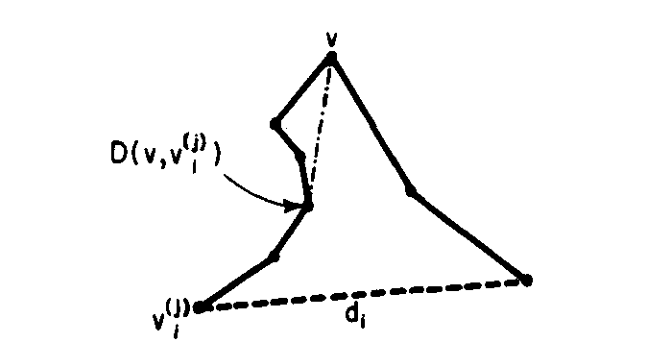
\includegraphics[width=0.7\textwidth]{Images/BTL[image]/lee_fig2.png} % Replace with your image file and path
  \caption{Minh họa về sự lồi vào trong của $D\left(s,v^{(j)}_i\right)$.}
  \label{fig:2} % Optional label for referencing
\end{figure} 





Tổng quát đối với $D_i$, các chuỗi tách ra tại đỉnh $v$ nào đó được gọi là \textit{đỉnh phễu}\footnote{Từ nguyên: cusp} của hai chuỗi lồi vào trong. Chú ý rằng một trong hai chuỗi có thể rỗng nhưng không thể cả hai vì $v^{(1)}_i \ne v^{(2)}_i$. Nếu $D\left(v, v^{(1)}_i\right)$ rỗng thì thì $D\left(v,v^{(2)}_i\right) = d_i$.
\newpage
Thuật toán xây dựng $D_1,D_2,\cdots,D_p$ và cuối cùng $D\left(s,t\right)$. Chi tiết:

\begin{algorithm}
\caption{Xây dựng chuỗi $D_i$}
\begin{algorithmic}
    \STATE \textbf{Ban đầu:} nối $s$ với $v^{(1)}_1$ và $v^{(2)}_1$ để tạo $D_1$.
    \STATE \textbf{Tổng quát:} Để tạo ra $D_{i+1}$ từ $D_i$:
    \STATE Gọi $v$ là đỉnh phễu của $D_i$, tại đỉnh hai chuỗi $\overline{u_a u_{a+1} \cdots u_b}$ và $\overline{u_a u_{a-1} \cdots u_0}$ tách ra, $v = u_a, v^{(1)}_i = u_b, v^{(2)}_i = u_0$. Không mất tính tổng quát: $v^{(1)}_i = v^{(1)}_{i+1}$. Bắt đầu từ $u_0$, gọi $j$ là số nguyên nhỏ nhất mà $\overline{v^{(2)}_{i+1} u_j}$ trở thành \textit{đường hỗ trợ}\footnotemark của đường biên của $R_i$. Xét hai trường hợp:
    \begin{itemize}
        \item [(i)] $j \leq a$. Xóa tất cả cạnh $\overline{u_l u_{l+1}}, 0 \leq l \leq j -1$ và thêm cạnh $\overline{u_j v^{(2)}_{i+1}}$.
        \item [(ii)] $j > a$. Xóa tất cả cạnh $\overline{u_l u_{l+1}}, 0 \leq l \leq j -1$ và thêm cạnh $\overline{u_j v^{(2)}_{i+1}}$; $u_j$ trở thành đỉnh phễu mới của $R_{i+1}$.
    \end{itemize}

    \STATE \textbf{Bước cuối:} Khi xây dựng xong $D_{n-3}$, ta xem như có thêm một đường chéo chứa $t$ (đường chéo $d_{n-2}$) và áp dụng lại bước Tổng quát ở trên.
    \STATE \textbf{Kết quả:} $D\left(s,t\right)$
\end{algorithmic}
\end{algorithm}

\begin{figure}[h] % h: here, t: top, b: bottom, p: page of floats
  \centering
  %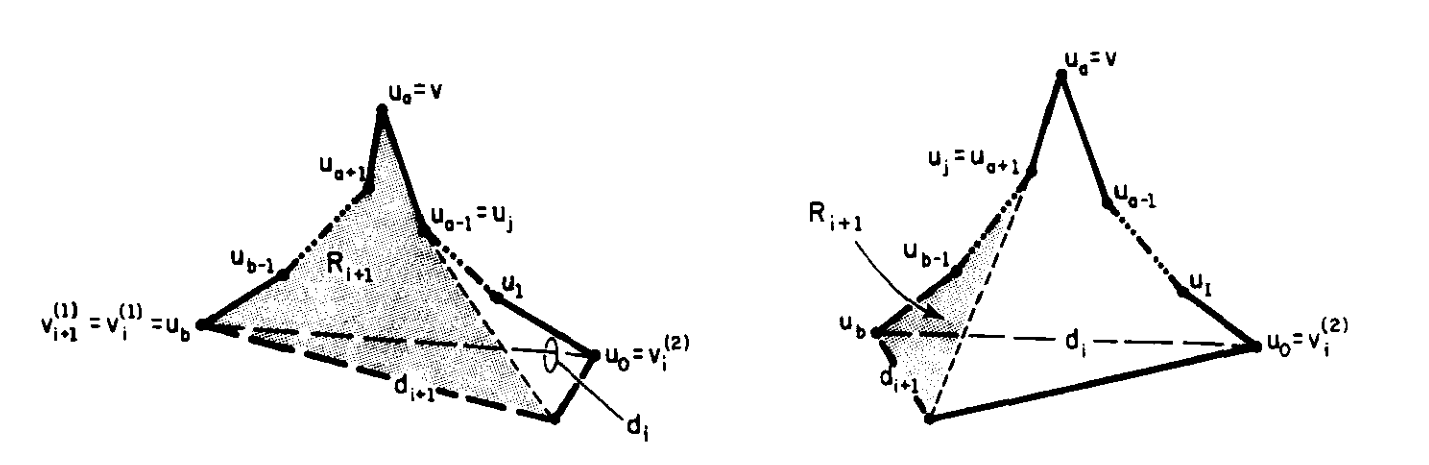
\includegraphics[width=0.95\textwidth]{Images/BTL[image]/lee_fig3.png} % Replace with your image file and path
 \begin{tikzpicture}[scale = 0.45]
    \coordinate (a) at (0,0);
    \coordinate (b) at (2, 1);
    \coordinate (c) at (4, 3.5);
    \coordinate (d) at (4.75, 5.5);
    \coordinate (e) at (5.5, 2.5);
    \coordinate (f) at (7.5, 1);
    \coordinate (g) at (10, -0.25);
    \coordinate (h) at (9, -2);
    \fill[lightgray, opacity = 0.5] (a) -- (b) -- (c) -- (d) -- (e) -- (h) -- cycle;
    \filldraw[black] (a) circle (2pt) node[left] {$v_{i+1}^{(1)} = v_i^{(1)} = u_b$};
    \filldraw[black] (b) circle (2pt) node[anchor = south east] {$u_{b-1}$};
    \filldraw[black] (c) circle (2pt) node[left] {$u_{a+1}$};
    \filldraw[black] (d) circle (2pt) node[above] {$u_a = v$};
    \filldraw[black] (e) circle (2pt) node[right] {$u_{a-1} = u_j$};
    \filldraw[black] (f) circle (2pt) node[anchor = south west] {$u_1$};
    \filldraw[black] (g) circle (2pt) node[right] {$u_0 = v_i^{(2)}$};
    \filldraw[black] (h) circle (2pt);
    \draw[thick] (a) -- (b);
    \draw[thick, dash dot] (b) -- (c);
    \draw[thick] (c) -- (d) -- (e);
    \draw[thick, dash dot] (e) -- (f);
    \draw[thick] (f) -- (g) -- (h);
    \draw[densely dashed] (e) -- (h);
    \draw[dashed] (h) -- (a) node[midway, below] {$d_{i+1}$};
    \draw[dashed] (a) -- (g);
    \draw (3,1) node[right] {$R_{i+1}$};
    \draw[thick] [latex-] (8.5, 0) to [bend left] (10, 1);
    \draw (10,1) node[right] {$d_i$};
    \draw (5, -2) node[below] {(i)};
    \draw[white] (0,-4) circle (2pt);
\end{tikzpicture}
\begin{tikzpicture}[scale = 0.45]
    \coordinate (a) at (0,0);
    \coordinate (b) at (1.75, 1.25);
    \coordinate (c) at (3, 3.25);
    \coordinate (d) at (4, 6);
    \coordinate (e) at (5, 3);
    \coordinate (f) at (7, 1);
    \coordinate (g) at (8.5, 0);
    \coordinate (h) at (1, -2);
    \fill[lightgray, opacity = 0.5] (a) -- (b) -- (c) -- (h) -- cycle;
    \filldraw[black] (a) circle (2pt) node[left] {$u_b$};
    \filldraw[black] (b) circle (2pt) node[anchor = south east] {$u_{b-1}$};
    \filldraw[black] (c) circle (2pt) node[left] {$u_j = u_{a+1}$};
    \filldraw[black] (d) circle (2pt) node[above] {$u_a = v$};
    \filldraw[black] (e) circle (2pt) node[right] {$u_{a-1}$};
    \filldraw[black] (f) circle (2pt) node[anchor = south west] {$u_1$};
    \filldraw[black] (g) circle (2pt) node[right] {$u_o = v_i^{(2)}$};
    \filldraw[black] (h) circle (2pt);
    \draw[thick] (a) -- (b);
    \draw[thick, dash dot] (b) -- (c);
    \draw[thick] (c) -- (d) -- (e);
    \draw[thick, dash dot] (e) -- (f);
    \draw[thick] (f) -- (g) -- (h);
    \draw[dashed] (a) -- (h) node[midway, left] {$d_{i+1}$};
    \draw[dashed] (a) -- (g) node[midway, above] {$d_i$};
    \draw[densely dashed] (c) -- (h);
    \draw[thick, latex-] (1.5, 0.5) to [bend left] (3.6, 2) node[right] {$R_{i+1}$};
    \draw (5, -2) node[below] {(ii)};
    \draw[white] (-2,0) circle (2pt);
    \draw[white] (0,-4) circle (2pt);
\end{tikzpicture}
 
  \caption{Hai trường hợp của bước tổng quát.}
  \label{fig:3} % Optional label for referencing
\end{figure} 



\footnotetext{Từ nguyên: supporting line. \textit{l} là đường hỗ trợ của một đường cong \textit{C} nếu nó có một điểm chung với \textit{C} và \textit{C} nằm toàn bộ ở một phía của \textit{l}}

\hspace{15cm}

Tính đúng đắn của thuật toán dựa trên nhận xét sau: Với mọi $u$ trong tam giác $R_{i+1}$ xác định bởi hai đường chéo $d_i, d_{i+1}$, đường đi ngắn nhất từ $s$ đến $u$ đi qua $v$ là đỉnh phễu của $D_i$. Hiển nhiên đúng với $i = 1, v=s$. Ta đi chứng minh bằng quy nạp như sau:

\begin{proof}
    giả sử đúng tới $1, \cdots, i -1$; xét hai chuỗi $D\left(v, v^{(1)}_i\right), D\left(v, v^{(2)}_i\right)$. Nếu một trong hai chuỗi là rỗng, chuỗi còn lại sẽ bao gồm $d_i$ với $v$ trở thành đỉnh của $d_i$. Trong trường hợp này, đường đi ngắn nhất từ $s$ tới $u$ phải là đoạn ngắn nhất của $D(s,v)$ và đoạn thẳng $\overline{vu}$, và hoàn tất chứng minh. Nếu cả hai chuỗi đều không rỗng, xét cạnh kề với đỉnh $v$ trên bất kỳ chuỗi con nào. Vì $P$ là sleeve, ít nhất một trong số chúng là đường chéo của $P$ (kể cả khi nó không phải đường chéo có được từ thuật toán tam giác hóa $P$). Gọi $\overline{v v'}$ là đường chéo và $\overline{v v^{"}}$ không phải đường chéo. Bởi vì sự lồi vào trong của hai chuỗi, các tia tạo bởi $\overline{v v'}$ và $\overline{v v^{"}}$ cắt $R_{i+1}$ thành ba phần. Điểm $u$ sẽ thuộc một trong ba phần này; cả ba trường hợp đều tương tự nhau. Giả sử đường ngắn nhất từ $s$ tới $u$ là chuỗi $l(s,u)$ không đi qua $v$ mà thay vào đó cắt $\overline{v v^{'}}, \overline{v v^{"}}$ tại $p \neq v, p_1 \neq v$. Theo định nghĩa đường đi ngắn nhất:    
    \[ length\left(l(s,p)\right) + length\left(l(p,p_1)\right) < length\left(D(s,v)\right) + length\left(\overline{v p_1}\right)  \]
    theo bất đẳng thức tam giác: 
    \[ length\left(D(s,v)\right) + length\left(\overline{vp}\right) - length\left(l(s,p)\right) > 0 \]
    Từ đó: 
    \[ length\left(D(s,v)\right) + length\left(\overline{vv'}\right) > length\left(l(s,p)\right) + length\left(\overline{pv'}\right) \]
    Trường hợp này mâu thuẫn với trường hợp đầu là đường ngắn nhất từ $s$ tới $v'$ là qua $v$.
\end{proof}

\newpage

\begin{figure}[h] % h: here, t: top, b: bottom, p: page of floats
  \centering
  %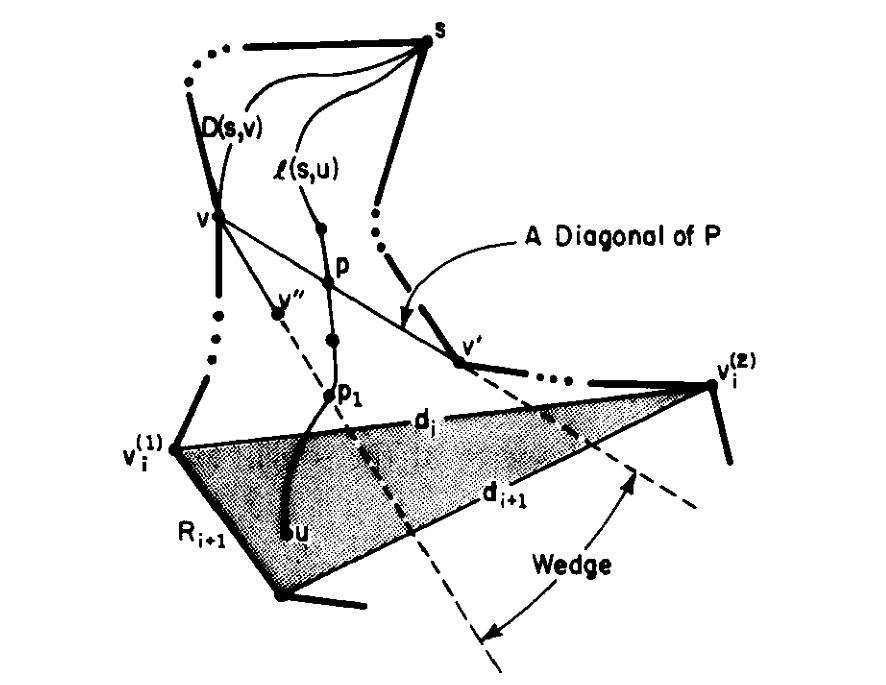
\includegraphics[width=0.65\textwidth]{Images/BTL[image]/lee_fig4.png} % Replace with your image file and path
  \begin{tikzpicture}[scale = 0.8]
  \coordinate (a) at (-1,0);
  \coordinate (b) at (1.25, 2.5);
  \coordinate (c) at (-0.5, 4);
  \coordinate (d) at (0.5, 6.75);
  \coordinate (e) at (3.4, 7.5);
  \coordinate (f) at (2, 5);
  \coordinate (g) at (3, 3);
  \coordinate (h) at (6, 2.5);
  \coordinate (i) at (8, -0.5);
  \coordinate (u) at (6, 0.7);
  \filldraw[lightgray, opacity = 0.5] (i) -- (a) -- (h) -- cycle;
  \draw[very thick] (a) -- (b) -- (c);
  \draw[very thick] (d) -- (e);
  \draw[semithick] (e) -- (f) node[midway, fill=white] {$D(s,v)$};
  \draw[very thick] (f) -- (g) -- (h) -- (i); 
  \draw[very thick] (a) -- +(1,-1);
  \draw[very thick] (i) -- +(1,-0.5);
  \draw[thick] (a) -- (h) node[midway, above] {$d_i$};
  \draw[thick] (a) -- (i) node[midway, below] {$d_{i+1}$};
  \draw[thick] (f) -- (b);
  \draw[thick, name path=vv, loosely dashed] (f) -- ($(f)!7cm!(b)$);
  \draw[thick, name path=vvv, loosely dashed] (f) -- ($(f)!7cm!(g)$);
  \draw[very thick] (e) -- ++(0.4, -0.8) ++(-0.16,-0.64) -- (f);
  \draw[very thick, dotted] (e)++(0.4, -0.8) .. controls (4,6.3) .. ++(-0.16,-0.64);
  \draw[semithick, name path=l] (e) .. controls (-1,5.8) and (1.5, 1) .. (u) node[near start, fill=white] {$l(s,u)$};
  \draw[very thick] (c) -- ++(0.84, 1.04) ++(0.25,0.64) -- (d);
  \draw[very thick, dotted] (c) ++(0.84, 1.04) .. controls (0.54,5.3) .. ++(0.25,0.64);

  \fill[black,name intersections={of=l and vv,by=p1}] (p1) circle (2pt) node[left] {$p$};
  \fill[black,name intersections={of=l and vvv, by=p2}] (p2) circle (2pt) node[anchor = south west] {$p_1$};
  \draw[thick, latex-] (1.7,4) to [bend right] ++(2, 0.7) node[anchor = south west] {Đường chéo của $P$};
  \fill[black] (e) circle (2pt) node[above] {$s$};
  \fill[black] (a) circle (2pt) node[left] {$v_i^{(2)}$};
  \fill[black] (f) circle (2pt) node[right] {$v$};
  \fill[black] (g) circle (2pt) node[anchor = south west] {$v''$};
  \fill[black] (b) circle (2pt) node[anchor = east] {$v'$};
  \fill[black] (h) circle (2pt) node[anchor = south west] {$v_i^{(1)}$};
  \fill[black] (i) circle (2pt); 
  \fill[black] (u) circle (2pt) node[above] {$u$}; 
  \draw (2.8,0.5) node {$R_{i+1}$};
  \draw[white] (-2,-2) circle (1pt);
\end{tikzpicture}
  \caption{Chứng minh đường đi ngắn nhất phải đi qua $v$.}
  \label{fig:4} % Optional label for referencing
\end{figure} 



Độ phức tạp của thuật toán: trường hợp (i) của bước Tổng quát cần thời gian không đổi (constant time); trường hợp (ii) có thể phải kiểm tra số lượng lớn đỉnh tuy nhiên mỗi điểm chỉ cần xem xét một lần trong quá trình kiểm tra và $P$ có $n-2$ đỉnh bên cạnh $s, t$ nên toàn bộ thuật toán chỉ cần $O\left(n\right)$. Tuy nhiên đó là khi giả sử rằng $P$ là sleeve; còn đối với bất kỳ một đa giác đơn $P$ gồm  $n$ đỉnh, để chuyển hóa thành sleeve, đầu tiên chúng ta phải tam giác hóa $P$: $O\left(n \log n \right)$; xây dựng dual tree $T$ cần $O\left(n\right)$.  Vậy nên toàn bộ quá trình có độ phức tạp $O\left(n \log n \right)$ với quá trình tam giác hóa chiếm nhiều thời gian nhất.
\newpage
\section{Triển khai thuật toán}
Toàn bộ code của thuật toán có thể tìm được ở link sau.
\href{https://github.com/tincuri/BTL_pptinh}{https://github.com/tincuri/BTL\_pptinh}
\subsection{Tam giác hóa}
Ở bước này nhóm em sử dụng thuật toán của ông Seidel\cite{} lấy source code từ trang web sau \cite[]. Ông ấy hình thang hóa đa giác và từ đó tách đa giác đó ra thành các monotone polygon. Từ đây ông dùng một thuật toán tham lam để tam giác hóa các đa giác con này. Độ phức tạp của thuật toán hình thang hóa là $O(n \text{log*}n)$ , với log* n là hàm log lặp\footnote{Từ nguyên: iterative logarithm} của n với tốc độ biến thiên rất chậm $\log_b^* (n) << \log_b(n)$ và trong thực tế thì gần tương đương với hàm hằng. Phần tam giác hóa của các monotone polygon con có độ phức tạp $O(n)$. Do đó độ phức tạp của thuật toán tam giác hóa là  $O(n \text{log*}n)$.
\subsection{Dual tree}
Ở phần này nhóm em sử dụng cấu trúc \textbf{Doubly connected edge list (dcel)} để biểu diễn hình dạng của đa giác đã được tam giác hóa.

Dcel là một kiểu dữ liệu dùng để biểu diễn một đồ thị phẳng $G(V,E)$ với $V=\{v_1,v_2,..v_n\}$ là là tập hợp các điểm của đồ thị và $E=\{e_1, e_2, ..e_n\}$ là tập hợp các cạnh kết nối giữa các điểm. 
dcel gồm 3 kiểu dữ liệu: half\_edge, vertex, face.  \textit{ half\_edge} như tên gọi của nó, là một cấu trúc dữ liệu gần giống như một nửa của một cạnh. Mỗi \textit{half\_edge} chứa các miền dữ liệu sau.
\begin{itemize}
  \item Twin, là một cạnh đối ngược với nó.
  \item Origin, là điểm bắt đầu của \textit{half\_edge}.
  \item Next, là một \textit{half\_edge} có điểm bắt đầu là điểm kết thúc của \textit{half\_edge} này.
  \item Prev, là một \textit{half\_edge} có điểm kết thúc là điểm bắt đầu của \textit{half\_edge} này.
  \item IncidentFace, là một \textit{face} mà có \textit{half\_edge} này làm bờ.
\end{itemize}

\textit{face} và \textit{vertex} có thêm một miền dữ liệu chứa một \textit{half\_edge} mà các dữ liệu đó kề.

Các miền dữ liệu của \textit{half\_edge} được diễn tả như hình sau.
\begin{figure}[h]
  \centering
  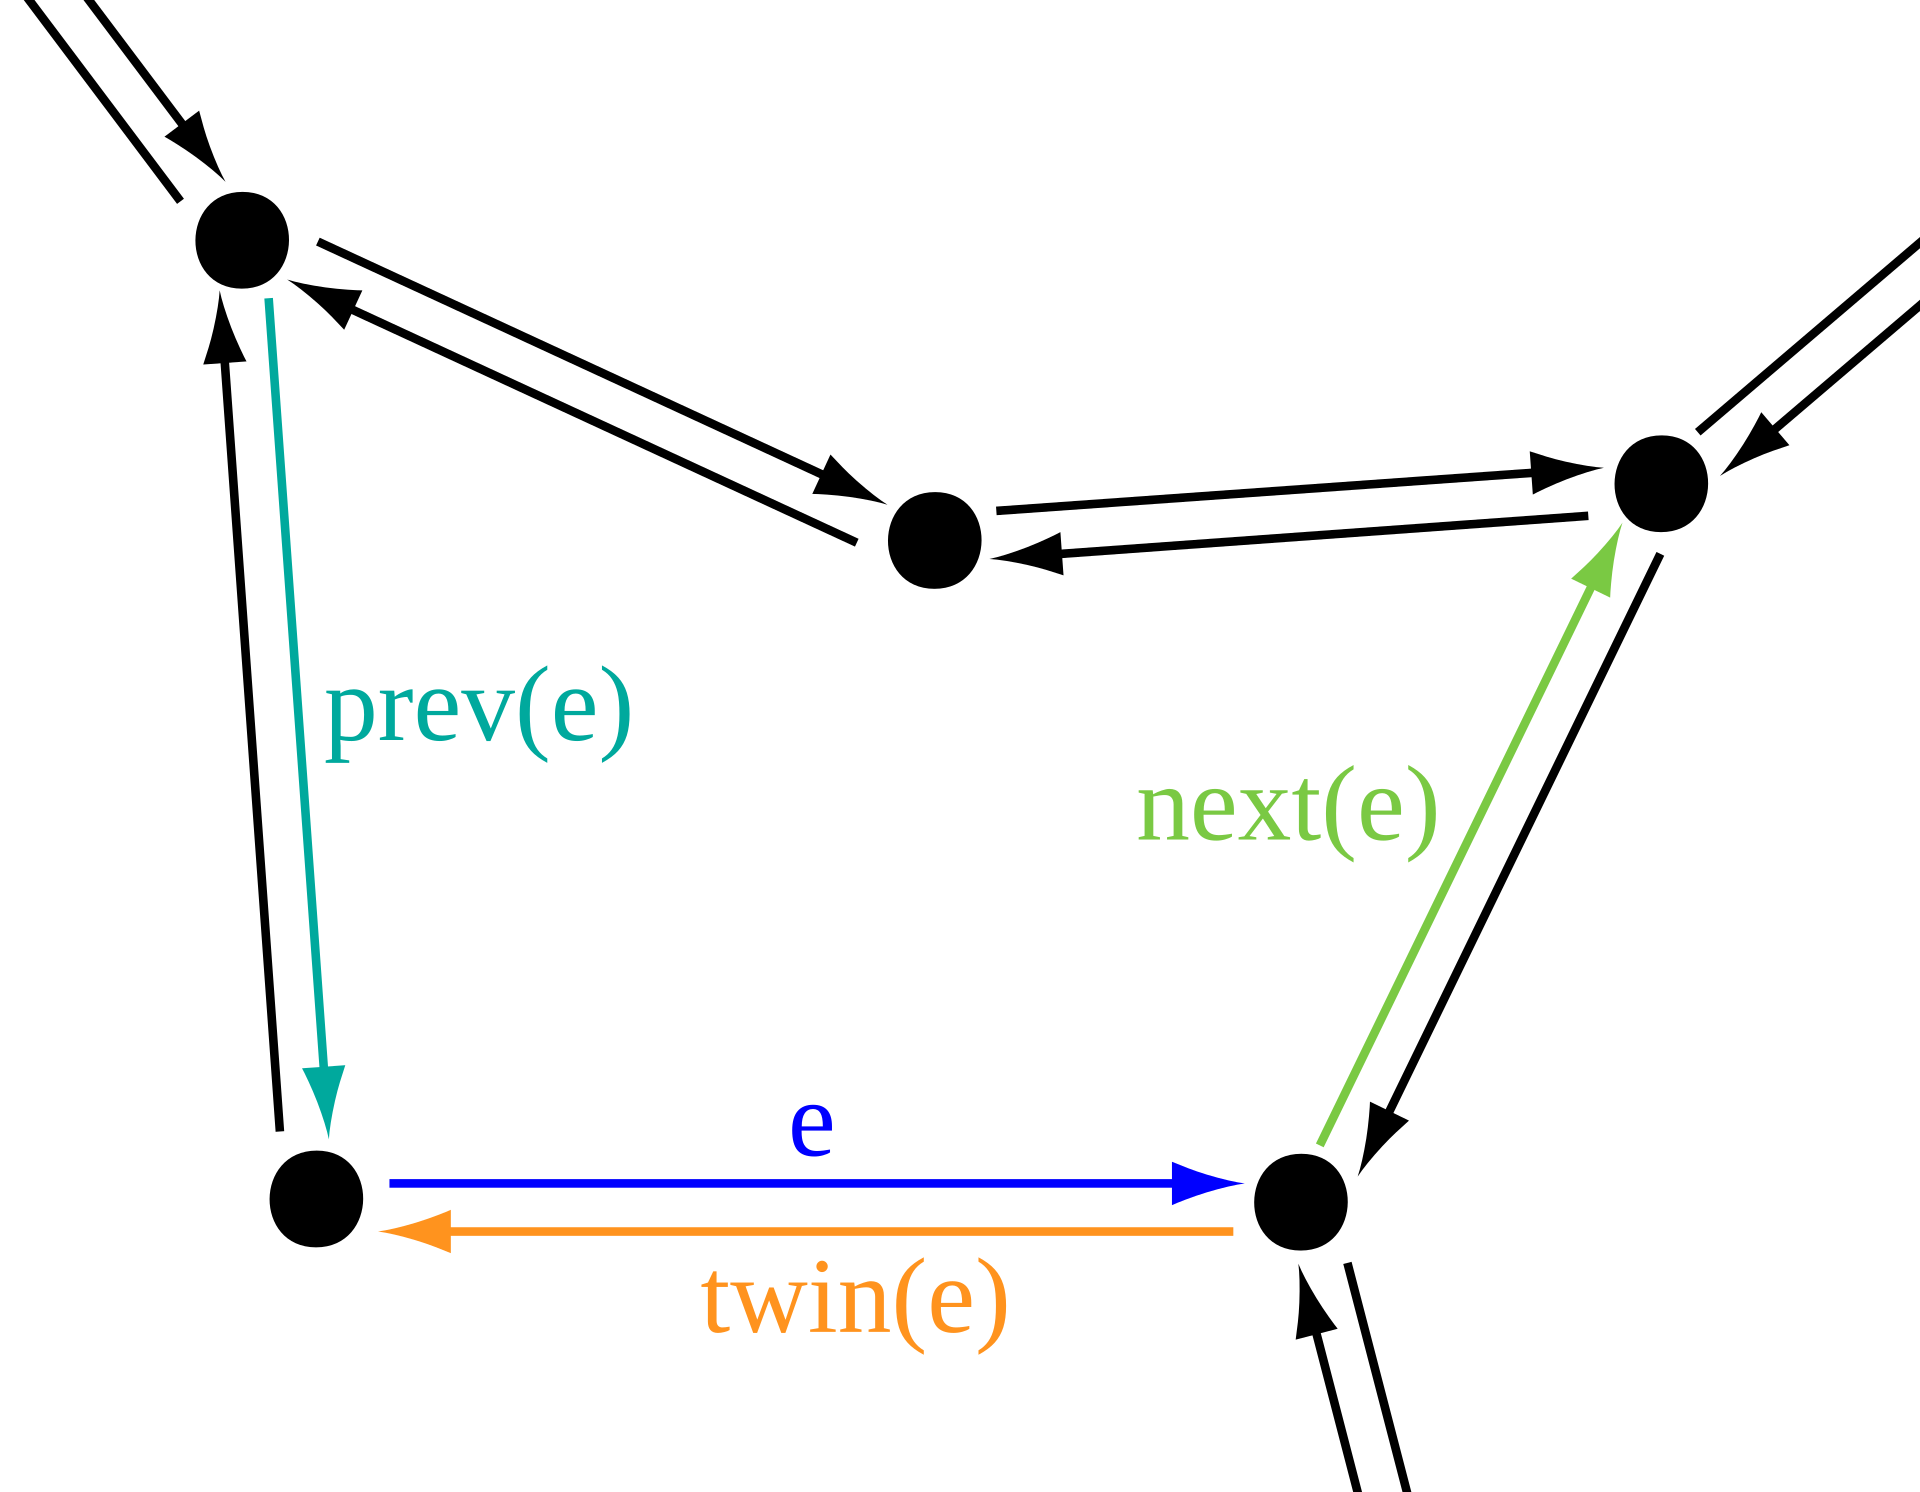
\includegraphics[width=0.45\textwidth]{Images/Dcel-halfedge-connectivity.svg.png}
\end{figure}

Dcel có thể được dựng dễ dàng như sau\cite{dcel}:
\begin{enumerate}
    \item Với từng điểm $v_i$ tạo một \textit{vertex} tương ứng.
    \item Với từng cạnh $e_i$ tạo hai \textit{half\_edge} tương ứng, đặt Origin cho 2 \textit{half\_edge} đó.
    \item Với từng \textit{vertex}, Sắp xếp các cạnh có nó là Origin theo chiều kim đồng hồ.
    \item Với hai \textit{half\_edge} $e_1, e_2$ kề nhau (trong thứ tự đã sắp xếp của một \textit{vertex} ở bước 3), gán $\text{Next}(\text{Twin}(e_1)) = e_2$ và $\text{Prev}(e_2) = \text{Twin}(e_1)$. 
    \item Lần lượt gán một \textit{face} cho các chuỗi \textit{half\_edge}
\end{enumerate}
Trong bước cuối, ta có thể lợi dụng việc gán mặt để tạo cho từ mặt một đỉnh trong đồ thị, và liên kết các đỉnh lại với nhau nếu hai mặt có chung một cạnh, mỗi liên kết có một miền dữ liệu là cạnh liên kết giữa hai mặt. Do đó ta có thể dựng được Dual tree của đa giác khi đang dựng dcel.

Như ta đã biết, để tam giác hóa một đa giác $n$ cạnh thì ta cần thêm $n-3$ đường chéo, mà mỗi đường chéo có 2 đỉnh. Do đó, trong trường hợp trung bình, mỗi đỉnh sẽ liên kết với khoảng 4 cạnh (thêm hai cạnh của đa giác ban đầu). Vì vậy độ phức tạp trung bình của thuật toán tạo DCEL trong trường hợp tam giác hóa là $O(n)$ nếu như bảo đảm các góc có số lượng cạnh liên kết tới nó gần ngang nhau. Trong trường hợp tệ nhất, tất cả các cạnh đều liên kết tới một góc, độ phức tạp của thuật toán khi này là $O(n\log n)$ do bước sắp xếp có độ phức tạp là $O(n\log n)$.
\subsection{Sleeve}
Bước đầu tiên, ta cần tìm vị trí của 2 điểm cần xét, ta có thể check\footnote{} xem điểm có nằm trong một tam giác bằng định hướng của nó với 3 đỉnh tam giác. Ta chỉ cần lặp qua các \textit{face} đến khi nào tìm được \textit{face} mà điểm đó nằm trong. Thuật toán có độ phức tạp là $O(n)$.

Với Dual Tree đã được tạo như trên, Nhóm em sử dụng Depth-first search (DFS) để tìm đường liên kết giữa 2 đỉnh tương ứng với 2 tam giác chứa 2 điểm. Đây chính là \textit{sleeve}. Từ đây ta rút ra được các đường chéo cần xét từ các liên kết. Độ phức tạp của DFS là $O(V+E)$ với $V = n$ là số đỉnh còn $E = n - 3$ là số cạnh. Do đó trong trường hợp này thuật toán tạo \textit{sleeve} có độ phức tạp là $O(n)$.

\subsection{Lee \& Preparata}
% hello ldm
% tui moi update anh vo latex de m can thi chen` vo result or smth
% oyasumi


\subsection{Kết quả}

\subsubsection{Độ phức tạp của các thuật toán}

\begin{table}[h]
    \centering
    \begin{tabular}{|c|c|c|}
    \hline
        \textbf{Thuật toán} & \textbf{Độ phức tạp trung bình}  & \textbf{Độ phức tạp tệ nhất}\\
    \hline
        Tam giác hóa & $O(n\text{log*}n)$ & $O(n\text{log*}n)$\\
    \hline
        Tìm Dual Tree & $O(n)$ & $O(n\log(n))$\\
    \hline
        Tìm Sleeve & $O(n)$ & $O(n)$ \\
    \hline
        Lee \& Preparata & $O(n)$ & $O(n)$\\
    \hline
    \end{tabular}
    \caption{Độ phức tạp của các thuật toán}
    \label{tab:complexity}

\subsubsection{Thời gian chạy thực tế}
\end{table}

\newpage
\section{Tổng kết}
\subsection{Nhận xét}
\subsection{Hướng phát triển}
Thay cho cấu trúc dcel, Ta cũng có thể dựng các cấu trúc khác như winged edge hay quad-edge cũng dùng để dựng một đồ thị phẳng và có thể có thời gian dựng ngắn hơn.

%%%%%%%%%%%%%%%%%OUTRO%%%%%%%%%%%%%%%%%%%
\section{Tài liệu tham khảo}
\begin{thebibliography}{9}
    \bibitem{Triangulate_linear}
    Bernard Chazelle. Triangulating a Simple Polygon in Linear Time. \textit{Discrete Comput. Geom.}, 6(5):485-524, 1991.

    \bibitem{Triangulate_nlogn}
    M. R. Garey, D. S. Johnson, F. P. Preparata, and R. E. Tarjan, Triangulating a simple polygon. \textit{Information Processing Lett}. 7 (1978) 175-179.

    \bibitem{Lee_paper_proof_lemma_1}
    O. Chein and L. Steinberg, Routing past unions of disjoint rectilinear barriers. \textit{Networks} \textbf{13} (1983) 389-398.

    \bibitem{dcel}
    \href{https://cs.stackexchange.com/questions/2450/how-do-i-construct-a-doubly-connected-edge-list-given-a-set-of-line-segments}{https://cs.stackexchange.com/questions/2450/how-do-i-construct-a-doubly-connected-edge-list-given-a-set-of-line-segments}
    
\end{thebibliography}

\newpage
\input{Outro/2-PhuLuc}
\end{document}


